\chapter{Fonctions, la suite}

Nous nous sommes déjà  intéressés aux fonctions affines, c'est-à-dire celles du type 

$$
f(x) = ax+b.
$$

À présent, nous allons étudier de plus près des fonctions un peu plus complexes, les fonctions du second degré et les fonctions homographiques.

\section{Fonctions du second degré}\label{seconddegre}

Une fonction du second degré est une fonction du type
$$
f(x) = ax^2 + bx + c.
$$

Notons que $a$ ne peut pas être égal à zéro. En effet, si tel est le cas, la fonction se transforme en une fonction affine et ce type a déjà été traité. Par contre, les coefficients $b$ et $c$ peuvent être zéro.

\begin{exemple}
Toutes les fonctions suivantes sont des fonctions du second degré, on a chaque fois identifié les coefficients $a$, $b$ et $c$ :
\newpage %mise en page des deux colonnes peu heureux
\begin{multicols}{2}
\begin{enumerate}
\item $f(x) = 2x^2 +3x -4$, $a=2$, $b=3$ et $c=-4$
\item $f(x) = -3x+x^2 +1$, $1=2$, $b=-3$ et $c=1$
\item $f(x) = -2x^2 + 4$, $a=-2$, $b=0$ et $c=4$
\item $f(x) = x^2 -x$, $a=1$, $b=-1$ et $c=0$
\item $f(x) = 42x^2$, $a=42$, $b=0$ et $c=0$
\end{enumerate}
\end{multicols}
\end{exemple}

\subsection{Zéros de fonction}

Comme nous l'avons déjà vu, les zéros de fonction sont les solutions de l'équation $f(x) = 0$. Puisqu'ici il s'agit d'une équation quadratique,
$$
ax^2 + bx + c = 0
$$
Or nous avons vu au chapitre~\ref{seconddegre} que les solutions sont données par
$$
\left\{
\begin{array}{lcl}
x_1 &=& \frac{-b-\sqrt{\Delta}}{2a}\\
&&\\
x_2 &=& \frac{-b+\sqrt{\Delta}}{2a}
\end{array}
\right.
$$

\subsection{Particularité : axe de symétrie et extremum}

Comme on peut le voir dans les graphiques de fonctions ci-dessous, les fonctions du second degré ont un axe de symétrie vertical. Nous allons essayer de deviner comment le trouver :

\begin{center}
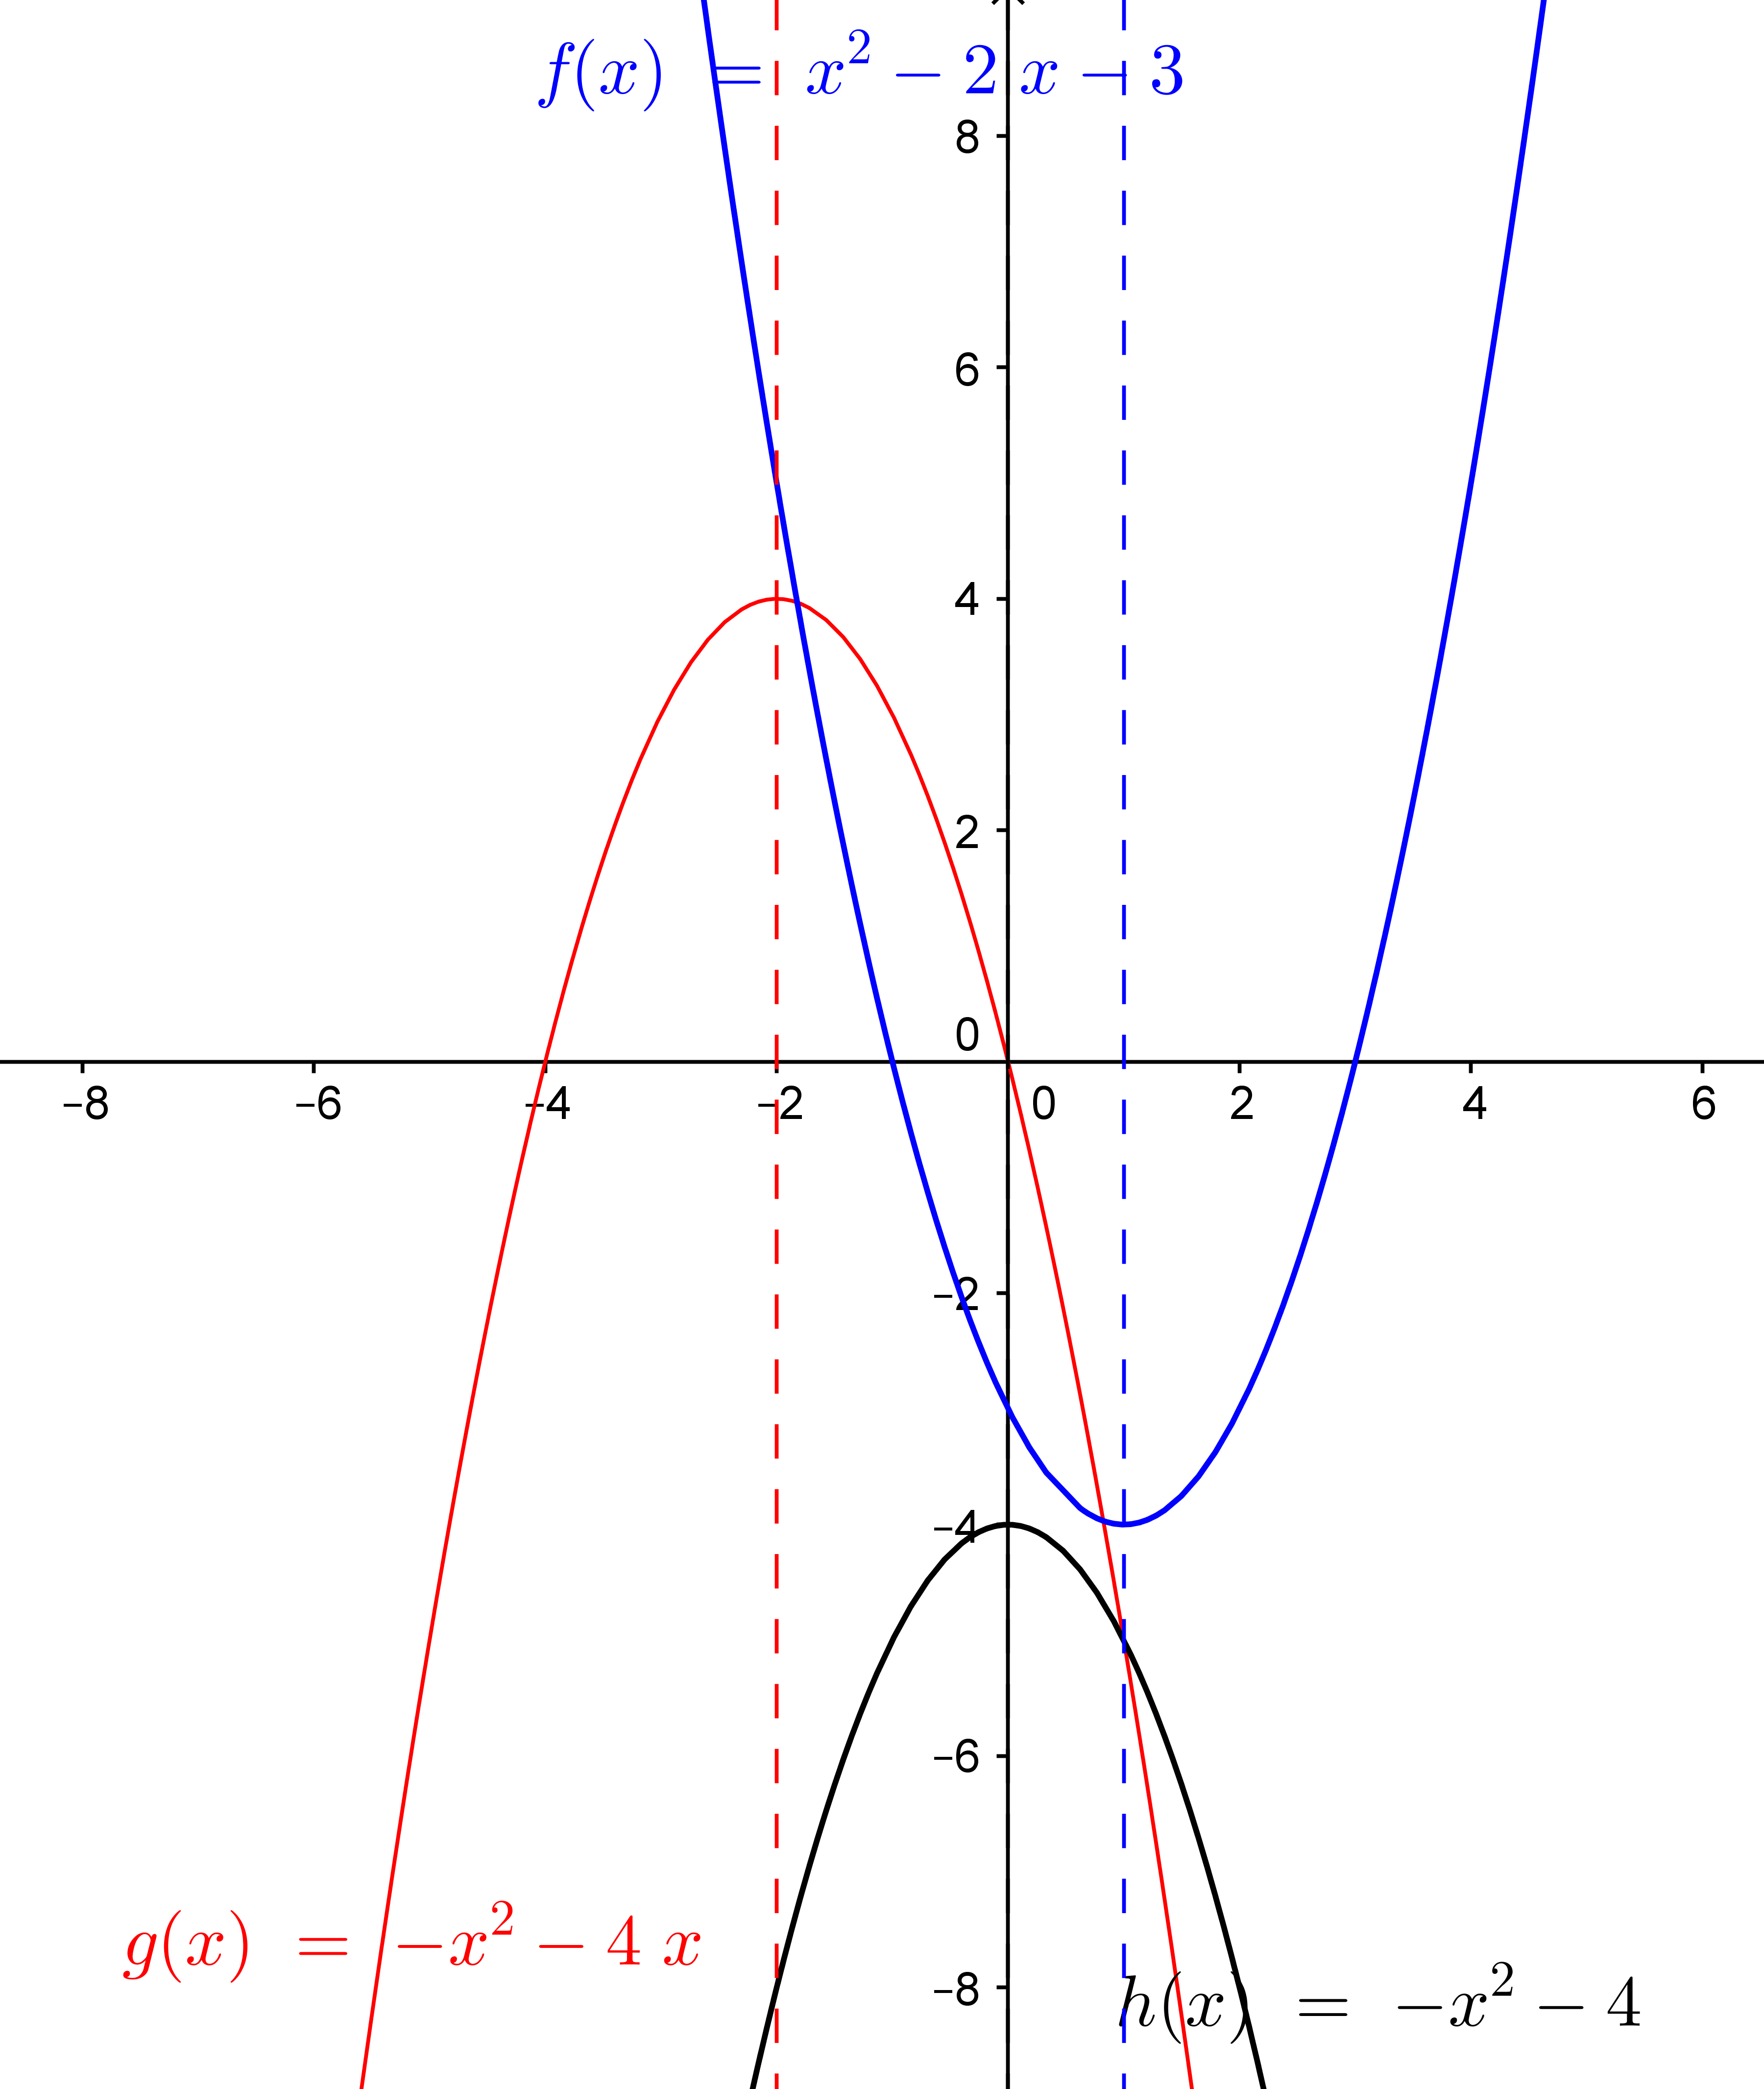
\includegraphics[width = 0.6\textwidth]{quadratique/quadratique.png}
\end{center}

Nous avons vu à la section précédente que les deux zéros de fonctions sont donnés par la formule 

$$
\left\{
\begin{array}{lcl}
x_1 &=& \frac{-b-\sqrt{\Delta}}{2a}\\
&&\\
x_2 &=& \frac{-b+\sqrt{\Delta}}{2a}
\end{array}
\right.
$$

Puisque la fonction est symétrique, l'axe doit passer au milieu des deux zéros de fonction, c'est-à-dire par
$$
\frac{x_1+x_2}{2} = \frac{\frac{-b-\sqrt{\Delta}}{2a}+\frac{-b+\sqrt{\Delta}}{2a}}{2} = \frac{-2b}{4a} = \frac{-b}{2a}
$$

\begin{proposition}
La fonction $f(x) = ax^2 + bx+c$ possède un axe de symétrie en $x= \frac{-b}{2a}$.
\end{proposition}

\begin{proof}
Le raisonnement pour les zéros de fonction marche aussi pour les fonctions qui ne coupent pas l'axe horizontal. On peut vérifier que pour $x_1<\frac{-b}{2a}$ et $f(x_1)$, alors le point symétrique $\left(x_1-\frac{b}{a};f(x_1)\right)$ est aussi sur la courbe, mais le calcul est laissé au lecteur ;-)

\end{proof}

Par ailleurs, on peut voir sur les tracés de courbes de fonctions que la fonction quadratique admet un \emph{extremum}\index{Extremum}, c'est-à-dire un point plus haut que tous les autres (maximum) ou plus bas que tous les autres (minimum). Intuitivement, cet extremum se trouve à l'intersection de l'axe de symétrie et de la courbe de la fonction, mais comme le dessin ne peut pas être aussi précis qu'un calcul, il pourrait aussi se trouver légèrement à gauche ou légèrement à droite.

\begin{proposition}
L'extremum sur $\R$ de la fonction $f(x) = ax^2 + bx + c$ se trouve en 
$$
\left(\frac{-b}{2a};\frac{-\Delta}{4a} \right),
$$
c'est-à-dire à l'intersection de la courbe de la fonction et de son axe de symétrie.
\end{proposition}

\begin{proof}
Nous allons démontrer cette proposition par l'absurde\index{démonstration par l'absurde} : on va supposer que l'extremum se trouve ailleurs, et on va arriver à une contradiction. Ainsi notre supposition est fausse et c'est son contraire qui est vrai. Par ailleurs, on peut aussi faire le raisonnement uniquement dans le cas d'un minimum, le cas d'un maximum étant le même à un mot près.

Supposons donc que l'extremum ne se trouve pas sur l'axe de symétrie, disons le point $(a;f(a))$. Ainsi grâce à ce même axe de symétrie, on peut trouver un autre point de l'autre côté de l'axe, disons $(b;f(b))$ qui est aussi un extremum, puisque ces deux points ont la même deuxième coordonnée, c'est-à-dire $f(a) = f(b)$. Mais comme il s'agit d'un maximum, tous les points de la courbe de $f$ dont l'abscisse se situe entre $a$ et $b$ doivent avoir une deuxième coordonnée inférieure ou égale à $f(a)$. Mais cela suppose donc que la fonction entre $a$ et $b$ fasse des "bosses" ou des "plats", ce qui est absurde car il s'agit d'une fonction du second degré.

Ainsi notre supposition était erronée et l'extremum ne peut se trouver que sur l'axe de symétrie.

Pour démontrer que la deuxième coordonnée est donnée par $\frac{-\Delta}{4a}$, il suffit de calculer l'image de $\frac{-b}{2a}$ de la fonction $f(x) = ax^2 + bx + c$, mais le calcul est laissé au lecteur.

\end{proof}

\subsection{Étude complète}

\begin{exemple}
Étudier complètement la fonction $f(x) = -x^2 -x+6$
			\begin{itemize}
				\item Axe de symétrie : $x=-\frac{1}{2}$
				\item Extremum : $(-\frac{1}{2}; \frac{26}{4})$
				\item Ordonnée à l'origine : $(0;6)$
				\item Zéros de fonction : $(-3;0),(2;0)$
				\item Signes et variations :
				$$
				\begin{array}{c|c|c|c|c|c|c|c|c|c}
				x&-\infty & & -3 & & -\frac{1}{2} & & 0 & & +\infty\\
				\hline
				f(x)& - & - & 0 & + & \frac{26}{4} & + & 0&-&-\\
				\hline
				& \nearrow & \nearrow & &\nearrow &\mbox{max}& \searrow & & \searrow & \searrow
				\end{array}
				$$
				\item
				
				\begin{center}
				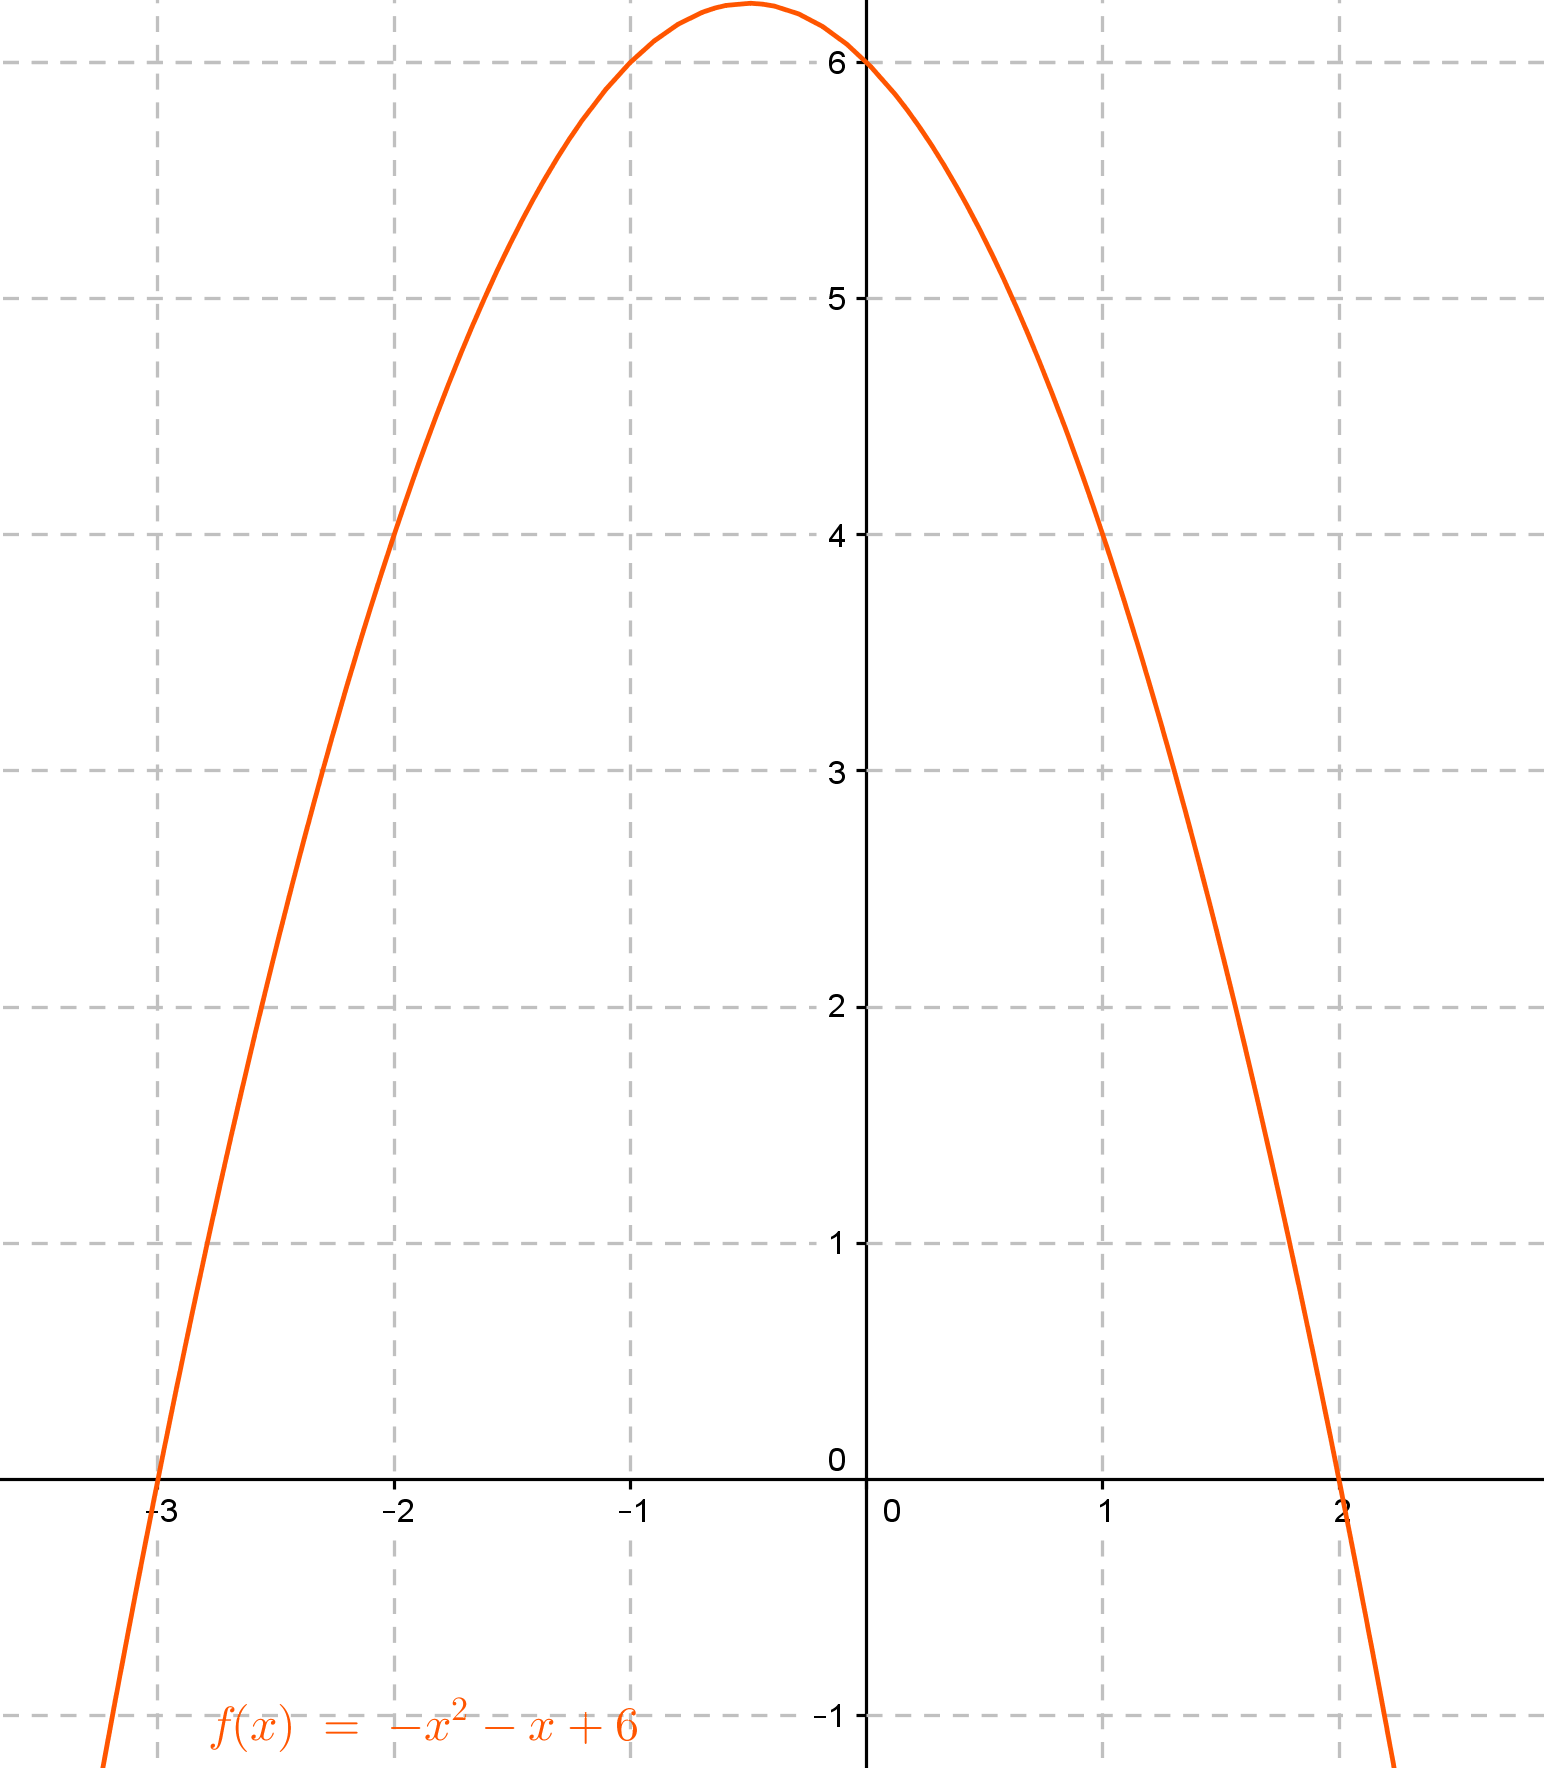
\includegraphics[width = 0.5\textwidth]{quadratique/fct_quadratique01.png}
				\end{center}
			\end{itemize}
\end{exemple}

\section{Fonctions homographiques}\label{homographique}

Une fonction homographique est une fonction du type 
$$
f(x) = \frac{ax+b}{cx+d}
$$

Notons que $c$ ne peut pas être égal à zéro. En effet, si tel est le cas, la fonction se transforme en une fonction affine et ce type a déjà été traité. Par contre, les coefficients $a$, $b$ et $d$ peuvent être zéro, mais pas $a$ et $b$ en même temps, car dans ce cas on aurait la fonction $f(x) = 0$ qui a déjà été étudiée elle aussi, ni $b$ et $d$ car le $x$ se simplifie alors.

\begin{multicols}{2}
\begin{exemple}
\begin{enumerate}
\item $$f(x) = \frac{2x-1}{x+3}$$
\item $$f(x) = \frac{3}{3x+1}$$
\item $$f(x) = \frac{3x}{x+1}$$
\item $$f(x) = \frac{2}{x}$$
\end{enumerate}
\end{exemple}
\end{multicols}

\subsection{Domaine de définition}

Contrairement aux autres fonctions déjà étudiées, les fonctions homographiques contiennent une opération qui peut être problématique : une division par un polynôme. En effet, dans le cas où l'image du dénominateur ($cx+d$) vaut zéro, l'image de la fonction est impossible car on ne peut pas diviser par zéro !

En d'autres termes, il faut enlever de l'ensemble de tous les nombres $\R$ celui dont la fonction ne peut donner d'image.

\begin{exemple}
$$
f(x) = \frac{2x-1}{x+3}
$$
Il ne faut pas que le dénominateur soit nul, c'est-à-dire dans ce cas, que 
$$
x+3 = 0 \ssi x=-3.
$$
On a donc comme domaine de définition 
$$
\R-\{-3\},
$$
c'est-à-dire qu'on peut rentrer n'importe quel nombre dans la fonction $f$ et trouver son image, sauf le nombre $-3$.
\end{exemple}

\subsection{Particularités : deux asymptotes}

Le terme \emph{asymptote} vient du grec : "a-" est un terme privatif, "-sym-" signifie "avec, ensemble" et "-ptote" le fait de tomber. Le terme "asymptote" signifie donc "qui s'approche sans rejoindre".

\subsubsection{Asymptote verticale}

Puisque le domaine de définition n'est pas tout $\R$, nous allons nous intéresser à ce qui se passe au voisinage du nombre exclu. Nous allons donc regarder ce qui se passe lorsque l'on fait rentrer des nombres qui s'approchent de plus en plus du nombre en question : 

\begin{exemple}
$$
f(x) = \frac{2x-1}{x+3}
$$
Faisons le tableau de correspondance qui s'approche de $-3$ par des nombres inférieurs :
$$
\begin{array}{|r|r|r|r|r|r|}
\hline
-4 & -3.5 & -3.1 & -3.01 & -3.001& -3.0001\\
\hline
9 & 16 & 72 & 702 & 7'002 & 70'002\\
\hline
\end{array}
$$
Puis par des nombres supérieurs :
$$
\begin{array}{|r|r|r|r|r|r|}
\hline
-2 & -2.5 & -2.9 & -2.99 & -2.999& -2.9999\\
\hline
-5 & -12 & -58 & -598 & -5'998 & -59'998\\
\hline
\end{array}
$$
Ainsi si l'on s'approche depuis des nombres inférieurs à $-3$, leur image devient de plus en plus grande, alors que si l'on s'approche par des nombres supérieurs, leur image devient de plus en plus petite (c'est-à-dire de plus en plus grande négativement)

On peut donc noter
$$
x\underset{x\rightarrow-3}{\overset{f}{\longrightarrow}} \infty
$$

On parle alors d'\emph{asymptote verticale} en $x=-3$, c'est-à-dire que lorsque $x$ se rapproche de $-3$, la courbe de la fonction va venir "se coller", être \emph{asymptotique} à la droite verticale $x=-3$.
\end{exemple}

\subsubsection{Asymptote horizontale}

Par ailleurs les fonctions homographiques ont un comportement intéressant lorsque $x$ devient très grand ou très petit (c'est-à-dire grand dans les négatifs).

\begin{exemple}
$$
f(x) = \frac{2x-1}{x+3}
$$
Faisons le tableau de correspondance avec des nombres de plus en plus grands :
$$
\begin{array}{|r|r|r|r|r|r|}
\hline
10 & 100 & 1'000 & 10'000 & 10^5& 10^6\\
\hline
1.46 &  1.93 & 1.99 & 1.999 & 1.9999&1.999993\\
\hline
\end{array}
$$
Puis avec des nombres de plus en plus petits :
$$
\begin{array}{|r|r|r|r|r|r|}
\hline
-10 & -100 & -1'000 & -10'000 & -10^5& -10^6\\
\hline
3 & 2.07 & 2.007 & 2.007 & 2.0001 & 2.000007\\
\hline
\end{array}
$$
Ainsi plus l'on rentre de nombres grands en valeur absolue, plus le résultat de la fonction se rapproche de $2$. On peut facilement l'expliquer : plus le nombre est grand, moins le $+1$ et le $-3$ n'ont d'importance dans le calcul. On peut donc noter

$$
\frac{2x-1}{x+3}\underset{x\rightarrow \infty}{\overset{f}{\longrightarrow}} \frac{2x}{x} = 2
$$

On parle alors d'\emph{asymptote horizontale} en $y = 2$, c'est-à-dire que lorsque $x$ se rapproche des infinis, la courbe de la fonction va venir "se coller", être \emph{asymptotique} à la droite horizontale $y=2$.
\end{exemple}

\subsection{Étude complète}

\begin{exemple}
$$h(x) = \frac{x+2}{2x-4}$$
			\begin{itemize}
				\item Domaine de définition : $\R-\{2\}$, asymptote verticale en $x=2$
				\item Asymptote horizontale en $y=\frac{1}{2}$
				\item Ordonnée à l'origine : $(0;-\frac{1}{2})$
				\item Zéros de fonction : $(-2;0)$
				\item Signes et variations :
				$$
				\begin{array}{c|c|c|c|c|c|c|c}
				x&-\infty & & -2 & & 2 & &  +\infty\\
				\hline
				f(x)& \frac{1}{2} & + & 0 & - & || & + &\frac{1}{2}\\
				\hline
				& \searrow & \searrow & &\searrow & & \searrow & \searrow
				\end{array}
				$$
				\item 
				\begin{center}
				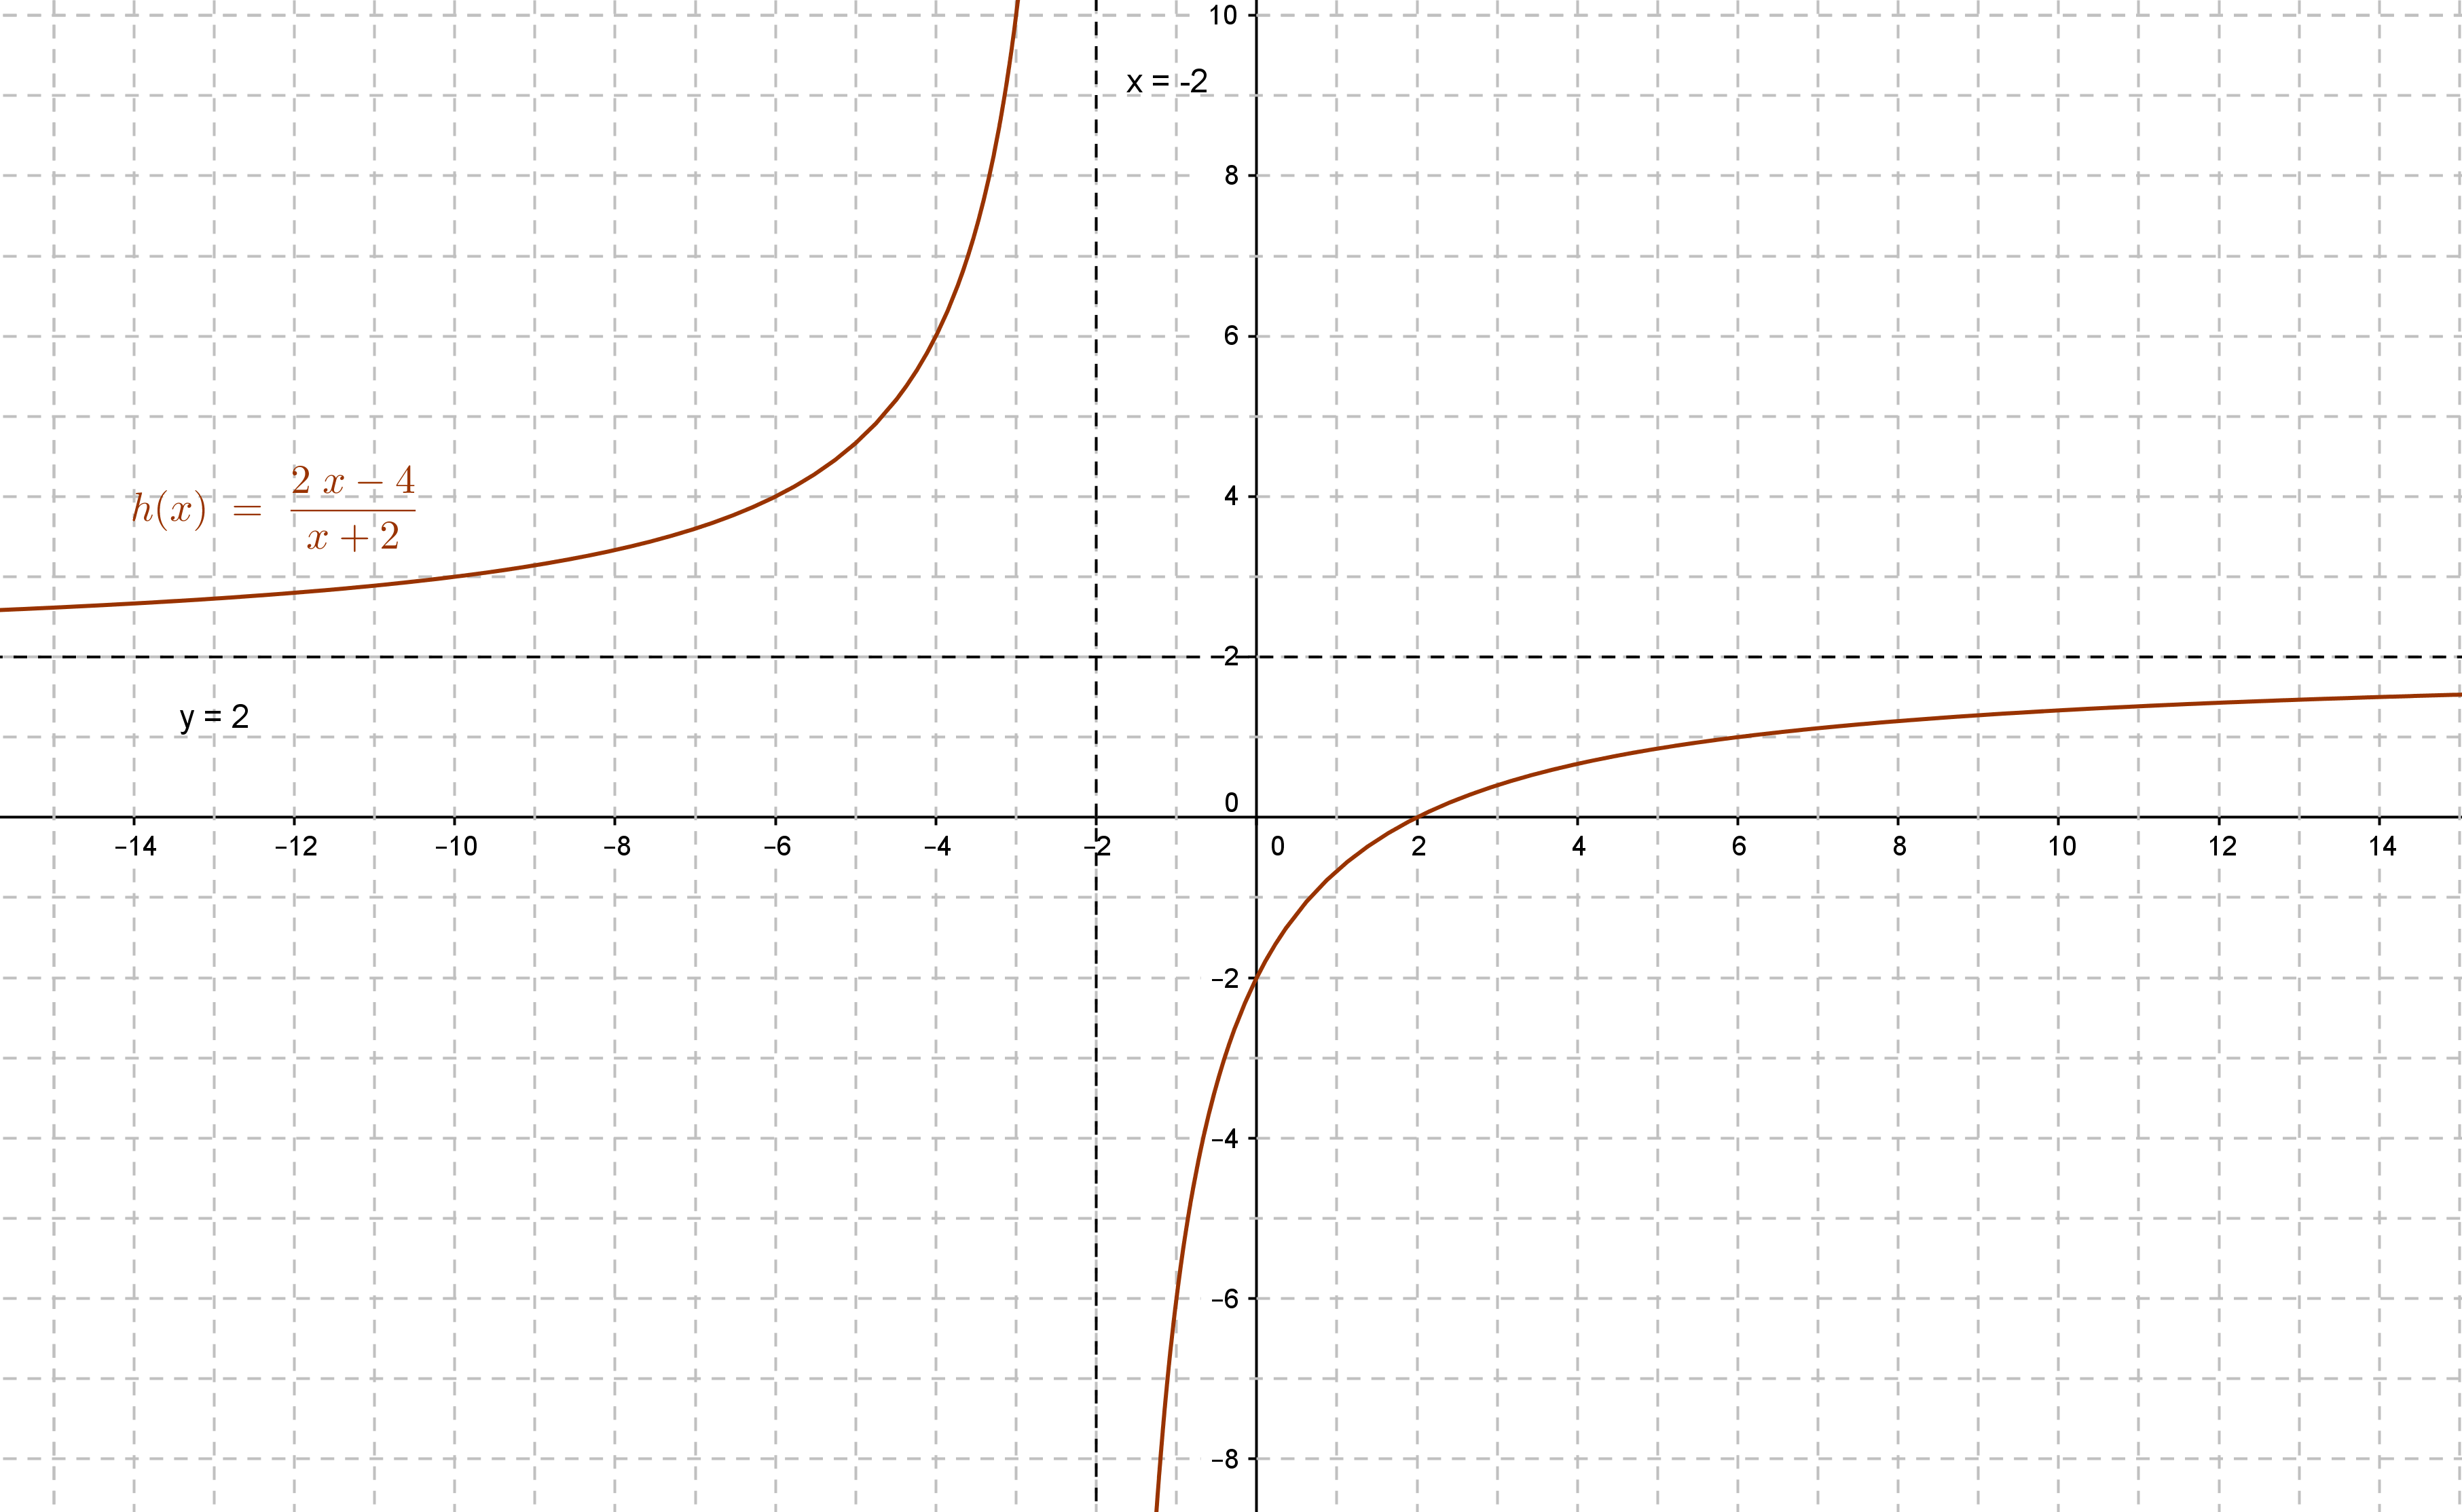
\includegraphics[width = 0.9\textwidth]{quadratique/homographique.png}
				\end{center}
			\end{itemize}
\end{exemple}

\section{Exercice}

\subsection{Fonctions quadratiques}

\begin{exercice}
\begin{multicols}{2}
Étudier les signes des trinômes suivants:
\begin{enumerate}
\item ${{x}^{2}}-7x+6$ 
\item $-3{{x}^{2}}+9x-6$ 
\item $4{{x}^{2}}-4x+1$ 
\item ${{x}^{2}}-x+1$ 
\item $-{{x}^{2}}+7x-12$
\item $-25{{x}^{2}}+10x-1$ 
\item $4{{x}^{2}}+16x+7$
\item ${{x}^{2}}$
\item $-{{x}^{2}}-5$
\item $-9{{x}^{2}}-12x-4$
\item $\left( 3x+1 \right)\left( x-2 \right)$
\item $\left( 6x-7 \right)\left( -x-5 \right)$
\item ${{\left( x+3 \right)}^{2}}-25$
\item $\left( 2x-1 \right)\left( x+3 \right)-\left( 2x-1 \right)\left( 3x-5 \right)$
\item ${{\left( 5-8x \right)}^{2}}$
\item ${{\left( x+2 \right)}^{2}}+5$
\end{enumerate}
\end{multicols}
\end{exercice}

\begin{exercice}
Calculer les coordonnées de l'extremum des fonctions suivantes, indiquer s'il s'agit d'un maximum ou d'un  minimum :
\begin{multicols}{2}
\begin{enumerate}
\item $f(x)=3{{x}^{2}}-2x+1$ 
\item $f(x)=-5{{x}^{2}}+x+2$ 
\item $f(x)={{x}^{2}}-x-20$ 
\item $f(x)=-\frac{{{x}^{2}}}{2}-3x+2$
\item $f(x)=-3{{x}^{2}}-8x+1$
\item $f(x)=\frac{{{x}^{2}}}{4}+\frac{x}{2}-3$
\item $f(x)=\frac{2{{x}^{2}}}{3}-\frac{x}{3}+4$
\item $f(x)={{x}^{2}}+x+1$
\item $f(x)=-\frac{3{{x}^{2}}}{25}+\frac{2x}{5}+2$
\end{enumerate}
\end{multicols}
\end{exercice}

\begin{exercice}
Étudier complètement les fonctions suivantes :
\begin{multicols}{2}
\begin{enumerate}
\item $f(x)={{x}^{2}}-4x+3$ 
\item $f(x)=-{{x}^{2}}+2x-8$ 
\item $f(x)={{x}^{2}}+2x+1$ 
\item $f(x)={{x}^{2}}+x+1$
\item $f(x)={{x}^{2}}$
\item $f(x)=-2{{x}^{2}}$
\item $f(x)={{x}^{2}}-4$
\item $f(x)=-{{x}^{2}}+6x-9$
\item $f(x)=-{{x}^{2}}-2$
\item $f(x)=-{{x}^{2}}+6x-5$
\item $f(x)=2{{x}^{2}}-6x+7$
\item $f(x)=2{{x}^{2}}-8x$
\item $f(x)=\frac{{{x}^{2}}}{4}-x-2$
\item $f(x)=\frac{{{x}^{2}}}{16}+\frac{x}{4}+\frac{1}{4}$
\end{enumerate}
\end{multicols}
\end{exercice}

\begin{exercice}
Trouver les coefficients m et n de la fonction $f(x)={{x}^{2}}+mx+n$ :
\begin{enumerate}
\item si elle admet pour $x=-2$ un minimum égal à 3
\item si elle admet 2 pour zéro de fonction et devient minimum pour $x=\frac{5}{4}$
\item si elle admet 1 pour zéro de fonction et un minimum égal à $\beta =-9$
\item si elle admet pour $x=2$ un minimum égal à 0
\item si elle admet pour zéros de fonction ${x}'=2$ et ${x}''=4$
\item si elle admet – 50 pour zéro de fonction et devient minimum pour $x=-55$
\item si elle admet une ordonnée à l'origine égale à 4 et un minimum égal à $\beta =-\frac{7}{4}$
\item si elle admet une ordonnée à l'origine égale à 49 et un zéro de fonction égal à 21
\end{enumerate}
\end{exercice}

\subsection{Problèmes d'optimisation}

\begin{exercice}
Quelle est la valeur maximale du produit de deux nombres si leur somme doit être égale à 35 ?
\end{exercice}

\begin{exercice}
Quelle est la valeur minimale du produit de deux nombres si leur différence doit être égale à 12 ?
\end{exercice}

\begin{exercice}
Sur la limite nord de son terrain, Louis a une montagne de roc qu'il peut utiliser pour former un des côtés d'un enclos rectangulaire pour ses chiens. Pour les trois autres côtés, il dispose de 80 m de clôture. Quelle est l'aire maximale qu'il peut donner à son enclos ?
\end{exercice}

\begin{exercice}
On a une longue pièce de fer-blanc de 30 cm de large. Le long de chacun des rebords, on redresse deux bandes de largeurs égales en les ramenant dans une position verticale formant ainsi une gouttière. Quelle doit être la largeur de ces bandes que l'on relève, si l'on veut que la gouttière ait une capacité maximale (aire d'une coupe transversale maximale) ?
\end{exercice}

\subsection{La fonction homographique}

\begin{exercice}
Calculer les asymptotes horizontales, les asymptotes verticales, les ordonnées à l'origine et les zéros de fonction des fonctions homographiques suivantes :
\begin{multicols}{2}
\begin{enumerate}
\item $f(x)=\frac{2x-3}{x-4}$
\item $f(x)=\frac{5x+2}{x+1}$
\item $f(x)=\frac{4-x}{2x-5}$
\item $f(x)=\frac{3x+5}{2x-1}$
\item $f(x)=\frac{2x}{3x+7}$
\item $f(x)=\frac{1}{x}$
\end{enumerate}
\end{multicols}
\end{exercice}

\begin{exercice}
Étudier complètement les fonctions homographiques suivantes :
\begin{multicols}{2}
\begin{enumerate}
\item $f(x)=\frac{x+1}{x-1}$
\item $f(x)=\frac{2x+1}{-x+2}$
\item $f(x)=\frac{x-3}{x-2}$
\item $f(x)=\frac{2x-4}{-x+4}$
\item $f(x)=\frac{4x+2}{x+1}$
\item $f(x)=\frac{-4x+6}{2x+1}$
\item $f(x)=\frac{6x-12}{-4x+4}$
\item $f(x)=\frac{2x-5}{x}$
\item $f(x)=\frac{1}{x}$
\item $f(x)=\frac{-5}{x}$
\end{enumerate}
\end{multicols}
\end{exercice}

\section{Corrigés}

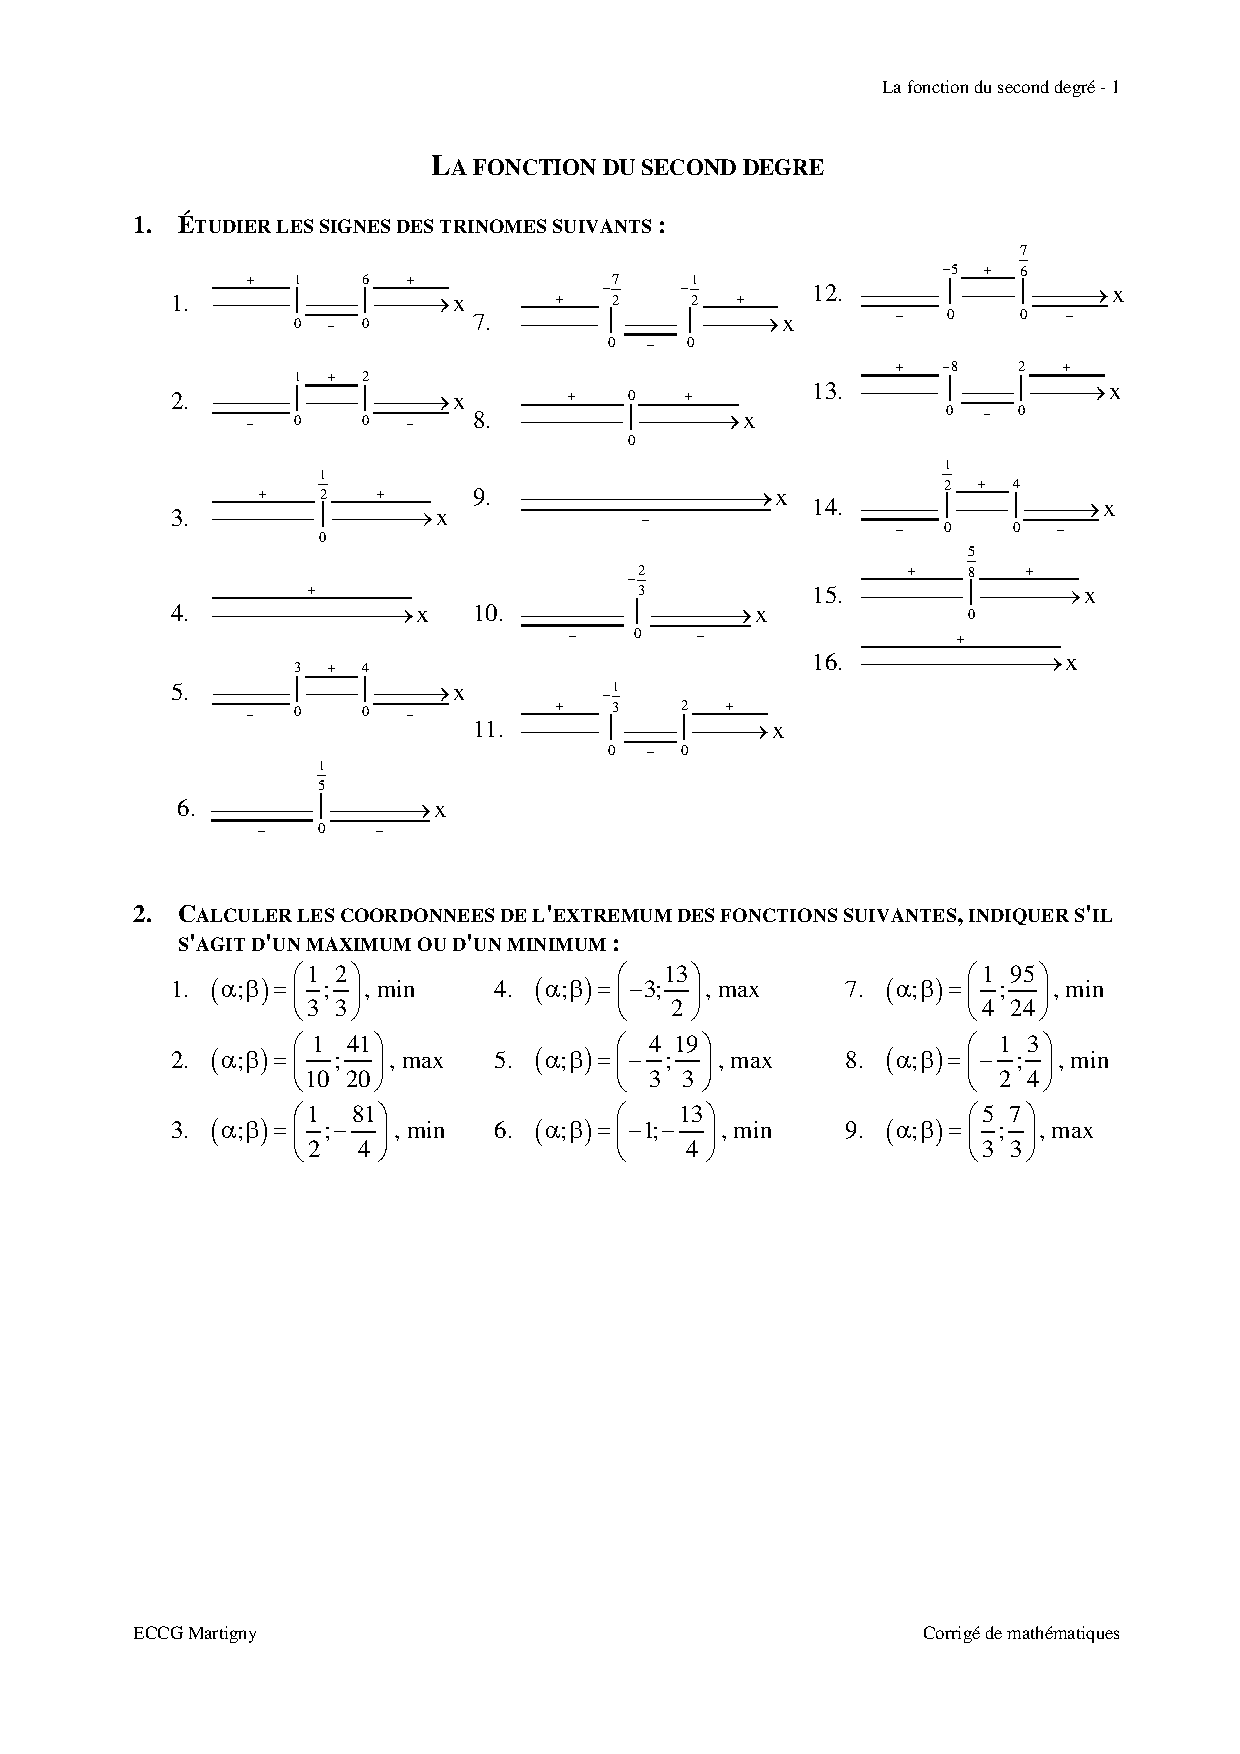
\includepdf[pages=1-8]{quadratique/second.pdf}
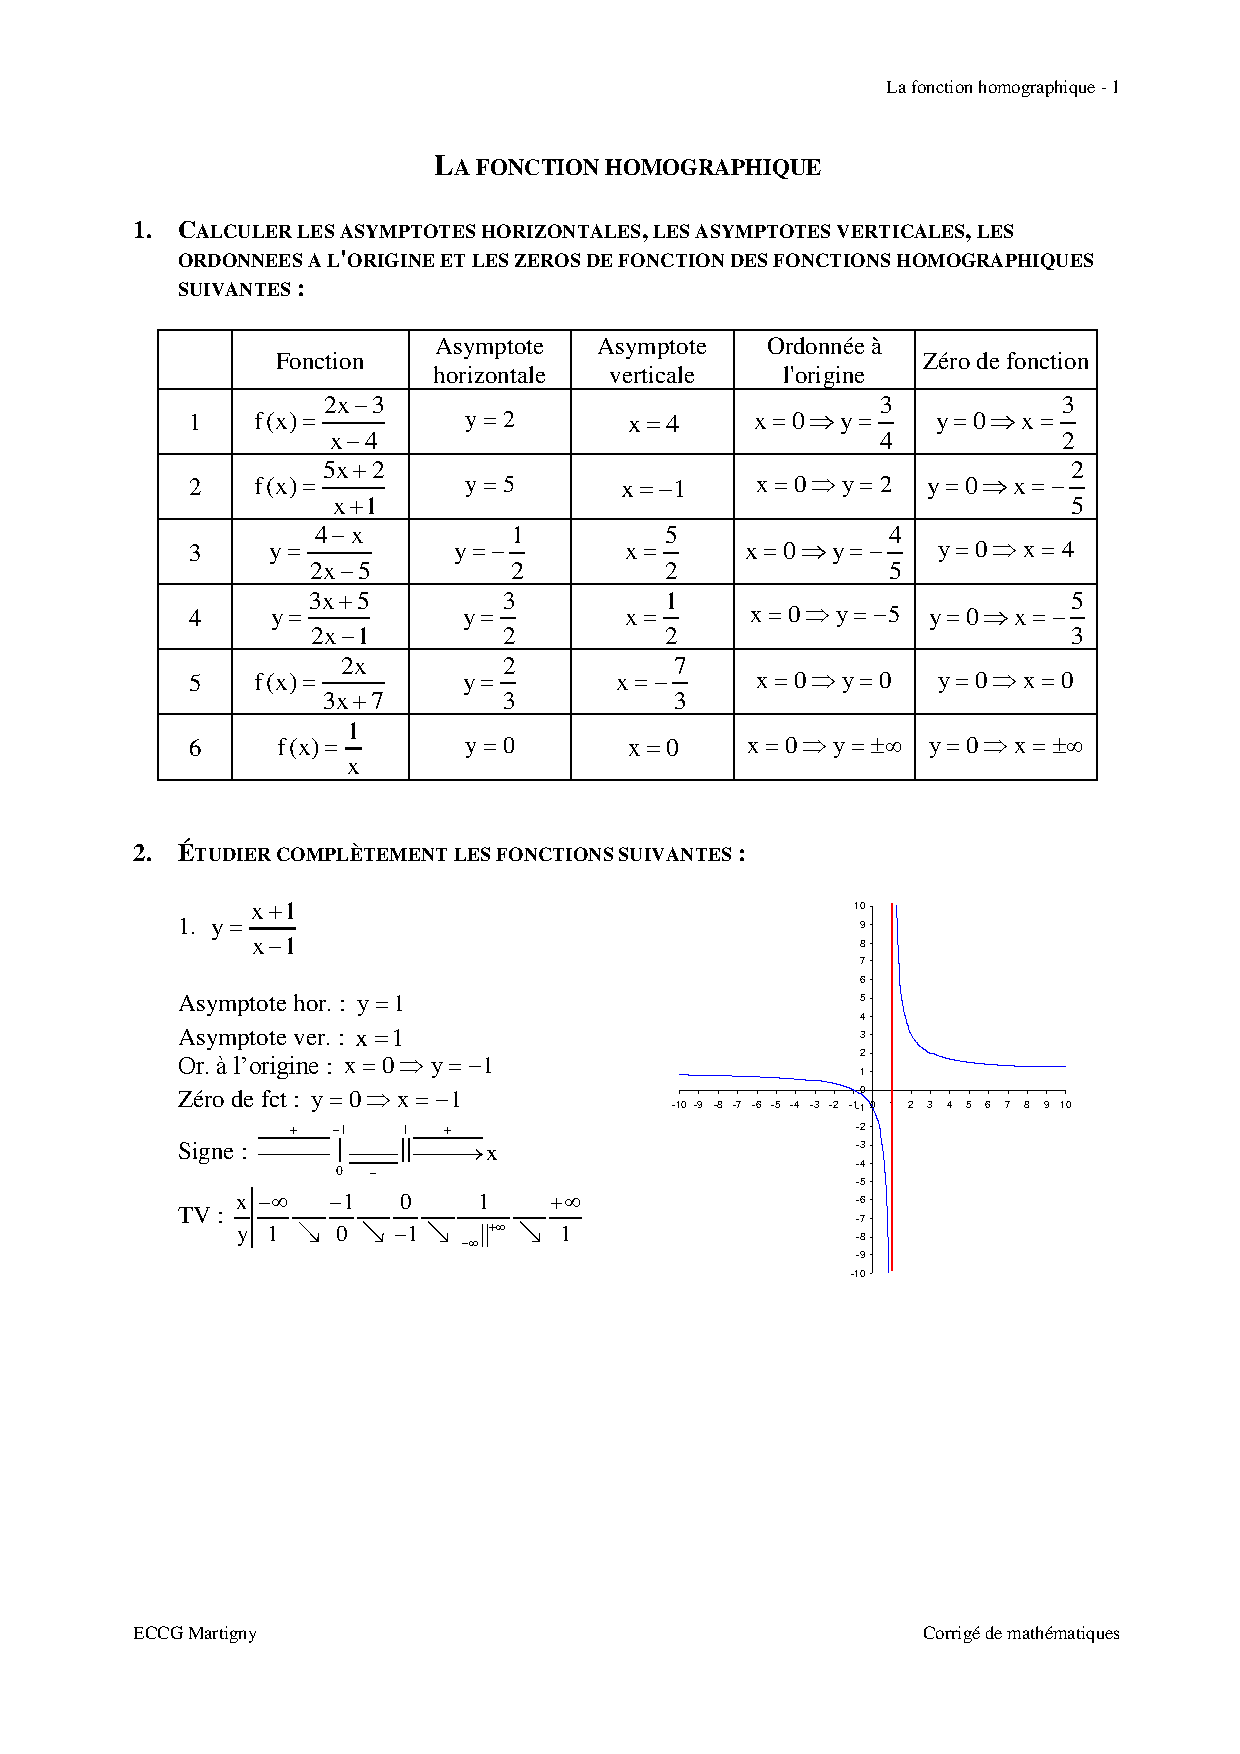
\includepdf[pages=1-4]{quadratique/homographique.pdf}